\documentclass[a4paper,12pt]{article}
\usepackage{times}
\usepackage[utf8]{inputenc}
\usepackage[brazil]{babel}
\usepackage[T1]{fontenc}
\usepackage{cite}
\usepackage{indentfirst}
\usepackage{url}
\usepackage{xcolor}
\usepackage{makecell}
\usepackage{multirow}
\usepackage{tabularx}
\usepackage{float}
\usepackage{graphicx}
% \usepackage{booktabs}
\definecolor{barblue}{RGB}{153,204,254}
\definecolor{groupblue}{RGB}{51,102,254}
\definecolor{linkred}{RGB}{165,0,33} 
\usepackage{geometry}
\usepackage[font=small,format=plain,labelfont=bf,up,textfont=it,up]{caption}
\usepackage{hyperref}

\restylefloat{table}
\setlength{\parindent}{1.2cm}
\setlength{\parskip}{.1cm}
\setlength{\oddsidemargin}{0.1cm}    
\setlength{\evensidemargin}{0.0cm}   
\setlength{\topmargin}{-1.2cm}       
\setlength{\headsep}{1.0cm}
\setlength{\textwidth}{15.5cm}
\setlength{\textheight}{24.2cm}
\renewcommand{\baselinestretch}{1.2}
\renewcommand{\labelitemi}{\tiny{\textbullet}}

\newcommand{\tabitem}{~~\llap{\textbullet}~~}

\begin{document}
\pagenumbering{roman}

\begin{titlepage}
\thispagestyle{empty}
\begin{center}
\large{\bf{IFPI - Instituto Federal de Educação, Ciência e Tecnologia do Piauí}} \\
% \large{\bf{Campus Teresina Central}} \\
% \large{\bf{Curso: Tecnólogo em Análise e Desenvolvimento de Sistemas}} \\
% \large{\bf{Disciplina: Projeto Integrador III}} \\
% \large{\bf{Professores: Fernando Santana e Ely Miranda}} \\
\end{center}
\vfill

\centering
\textbf{{\LARGE Documento de Visão - Vaga Livre}}  \\ \vspace{0.5cm}
\vfill

% \begin{tabular}{c}
%     \textit{Autores}\\
%     \hline
%     Igor Julliano \\
%     Kaíke Dias \\
%     Kelson Eduardo 
% \end{tabular}
% \vfill

\begin{center}
\large{\today}
\end{center}
\end{titlepage}

\pagenumbering{arabic}

% \begin{abstract}
% Em meio ao ritmo acelerado da vida urbana, encontrar vagas de estacionamento pode se transformar em um pesadelo. Dirigir em círculos por ruas congestionadas, lidar com filas em estacionamentos lotados e estacionar em locais apertados e mal iluminados são apenas alguns dos desafios que os motoristas enfrentam diariamente.

% É com o objetivo de libertar os motoristas da frustração de encontrar vagas de estacionamento que nasce o Vaga Livre, um aplicativo inovador que conecta motoristas a vagas disponíveis em tempo real, utilizando tecnologia de ponta para oferecer uma experiência de usuário impecável.

% Nossa missão é tornar o estacionamento mais fácil, eficiente e seguro para todos. Através do aplicativo, os motoristas terão acesso a uma série de recursos que facilitarão sua vida, como:

% \begin{itemize}
%     \item Visão em tempo real das vagas disponíveis em estacionamentos próximos: O aplicativo utiliza tecnologia de geolocalização para mostrar aos motoristas as vagas disponíveis em tempo real, permitindo que eles encontrem um lugar para estacionar rapidamente e sem estresse.
%     \item Reserva de vagas com antecedência: Para garantir ainda mais comodidade, os motoristas poderão reservar vagas com antecedência, evitando filas e a frustração de não encontrar um lugar para estacionar.
%     \item Pagamento rápido e seguro através do aplicativo: O aplicativo oferece diversas opções de pagamento rápido e seguro, como cartão de crédito, débito e pix, eliminando a necessidade de dinheiro em espécie e agilizando o processo de entrada e saída do estacionamento.
% \end{itemize}

% O aplicativo visa oferecer mais autonomia e agilidade aos motoristas, permitindo que eles percam menos tempo em interações de negociação ou burocracias com funcionários dos estacionamentos

% \end{abstract}

\vfill
\pagebreak
% TABLE OF CONTENTS
\tableofcontents{}
\pagebreak


%------------------------------------------------------------------------------------------------------
\section{Introdução}

A proposta deste documento é coletar, analisar e definir as necessidades e funcionalidades gerais do projeto \textbf{Vaga Livre}. Seu foco está nas necessidades dos usuários e no motivo da existência destas necessidades.

Seu escopo engloba a definição dos gestores do sistema, dos representantes dos usuários, seus problemas, necessidades e das características essenciais do sistema para o atendimento destes requisitos.

Termos e abreviaturas específicos podem ser encontrados.

\section{Posicionamento}

\subsection{Oportunidade de negócio}

O Vaga Livre resolve a frustração diária de encontrar vagas de estacionamento em centros urbanos congestionados, oferecendo uma experiência rápida, eficiente e sem estresse para os motoristas.

A demanda por soluções inteligentes de estacionamento \href{https://iot-analytics.com/smart-parking-market-report-2019-2023/}{cresce de maneira acentuada com o aumento da frota de veículos e a urbanização}, criando um mercado ávido por inovações como o Vaga Livre.

Desta forma o projeto almeja libertar os motoristas da frustração de encontrar vagas de estacionamento com um aplicativo inovador que conecta motoristas a vagas disponíveis em tempo real, utilizando tecnologia de ponta para oferecer uma experiência de usuário impecável.

\subsection{Declaração do problema}

\subsubsection{O problema}

Em meio ao ritmo acelerado da vida urbana, encontrar vagas de estacionamento pode se transformar em um pesadelo. Dirigir em círculos por ruas congestionadas, lidar com filas em estacionamentos lotados e estacionar em locais apertados e mal iluminados são apenas alguns dos desafios que os motoristas enfrentam diariamente. 

Assim temos que:

\begin{itemize}
    \item Encontrar vagas de estacionamento em centros urbanos congestionados é uma tarefa árdua e frustrante, consumindo tempo e gerando estresse para os motoristas.
    \item A procura por vagas pode levar até 30 minutos em média, causando atrasos, irritação e impacto na qualidade de vida das pessoas.
    \item A falta de vagas também contribui para o congestionamento urbano, poluição e emissão de gases poluentes.
\end{itemize}

\subsubsection{Quem ele afeta}

Aqueles afetados com este problema são:

\begin{itemize}
    \item Motoristas em geral, especialmente em grandes cidades.
    \item Pessoas com deficiência ou mobilidade reduzida.
    \item Famílias com crianças pequenas.
    \item Profissionais que dependem do carro para trabalhar, como motoristas de aplicativo, entregadores e vendedores.
    \item Empresas que operam frotas de veículos.
\end{itemize}


\subsubsection{O impacto do problema}

Com o problema, aqueles afetados experimentam

\begin{itemize}
    \item Perda de tempo e produtividade.
    \item Aumento do estresse e da ansiedade.
    \item Dificuldade de acesso a serviços essenciais, como saúde, educação e trabalho.
    \item Prejuízos financeiros para empresas e motoristas.
    \item Impacto negativo no meio ambiente.
\end{itemize}

\subsubsection{Solução}

Uma solução bem sucedida seria:

\begin{itemize}
    \item Uma plataforma que permite aos motoristas encontrar e reservar vagas de estacionamento com antecedência, de forma rápida e fácil.
    \item Um sistema que otimiza o uso dos espaços de estacionamento, reduzindo o tempo de procura por vagas e o congestionamento urbano.
    \item Uma solução que oferece segurança e comodidade aos usuários, com pagamento automático e monitoramento das vagas.
    \item Uma plataforma que contribui para a construção de cidades mais inteligentes e sustentáveis.
\end{itemize}


\section{Partes interessadas} % (fold)

\begin{table}[h!]
    \begin{tabularx}{\linewidth}{ | r | X | }
        \hline
        \bf{Representante} & \bf{Usuário} \\
        \hline
        \bf{Responsabilidades} & \tabitem{Encontrar e reservar vagas de estacionamento em tempo real.} \\
         & \tabitem{Visualizar a localização, o preço e a disponibilidade das vagas em tempo real.} \\
         & \tabitem{Pagar o estacionamento automaticamente através do aplicativo.} \\
         & \tabitem{Receber notificações quando uma vaga estiver disponível na área desejada.} \\
         & \tabitem{Monitorar o tempo de permanência no estacionamento.} \\
         & \tabitem{Avaliar os estacionamentos e compartilhar suas experiências com outros usuários. Observações:} \\
         & \tabitem{O aplicativo deve ser fácil de usar e intuitivo.} \\
         & \tabitem{O sistema de pagamento deve ser seguro e confiável.} \\
         & \tabitem{As informações sobre as vagas devem ser precisas e atualizadas em tempo real.} \\
        \hline
    \end{tabularx}
\end{table}


\begin{table}[h!]
    \begin{tabularx}{\linewidth}{ | r | X | }
        \hline
        \bf{Representante} & \bf{Próprietário do estacionamento} \\
        \hline
        \bf{Responsabilidades} &\tabitem{Definir o valor da tarifa de estacionamento.} \\
         & \tabitem{Definir e atualizar a disponibilidade das vagas em tempo real.} \\
         & \tabitem{Receber automaticamente os pagamentos das reservas online.} \\
         & \tabitem{Receber os pagamentos das reservas feitas presencialmente.} \\
         & \tabitem{Autorizar e gerenciar o acesso ao estacionamento de forma manual quando necessária.} \\
         & \tabitem{Relatar a ocupação das vagas feitas fora do aplicativo em tempo real para manter o catalogo atualizado.} \\
         & \tabitem{O sistema de pagamento deve ser seguro e confiável.} \\
         & \tabitem{As informações sobre as vagas devem ser precisas e atualizadas em tempo real.} \\
        \hline
    \end{tabularx}
\end{table}

\section{Ambiente do usuário}


\subsection{Ambiente físico}

    Não possui ambiente físico, apenas digital.

\subsection{Ambiente computacional}

    Os usuários que irão utilizar o sistema devem possuir um dispositivo móvel (celular, tablet) que possua acesso a internet para poder realizar o acesso ao sistema e realizar suas operações.

\section{Público alvo}

    O público-alvo do aplicativo Vaga Livre são motoristas frequentes que enfrentam as dificuldades da busca por vagas de estacionamento em seu dia a dia. Seja para encontrar um lugar rapidamente em áreas congestionadas, evitar o estresse de dar voltas desnecessárias ou simplesmente ganhar praticidade e otimizar seu tempo, o Vaga Livre oferece uma solução completa para quem busca tranquilidade e segurança ao estacionar seu veículo.

\section{Não Escopo do Vaga Livre}

\begin{enumerate}
\setlength\itemsep{-1.2em}
\item Foco no Proprietário do Estacionamento \\ 
    \tabitem{Aplicativo para Proprietários: No momento, o foco do projeto está em desenvolver um aplicativo completo e intuitivo para o usuário final, o motorista que busca uma vaga de estacionamento. O desenvolvimento de um aplicativo para proprietários de estacionamentos será considerado em etapas posteriores.} \\
    \tabitem{Gerenciamento por Proprietários: As funcionalidades relacionadas à gestão de vagas por parte dos proprietários, como atualização de disponibilidade, controle de acesso e preços dinâmicos, não serão contempladas nesta fase.} \\

\item Integração com Hardware \\
    \tabitem{Integração com Totens: A integração com totens de entrada e saída dos estacionamentos não está prevista no escopo inicial. O foco está na busca e reserva de vagas através do aplicativo.} \\
    \tabitem{Pagamento via App: O pagamento da tarifa de estacionamento não será realizado através do aplicativo nesta fase. Os métodos tradicionais de pagamento (dinheiro, cartão, etc.) serão utilizados.}\\

\item Expansão Geográfica \\
    \tabitem{Abrangência Nacional: A plataforma Vaga Livre será inicialmente lançada em uma região específica, com foco na validação do modelo de negócio e na otimização da experiência do usuário. A expansão para outras cidades e regiões será considerada em etapas posteriores.} \\

\item Visualização detalhada do Estacionamento \\
    \tabitem{Fotos e vídeos do local, mapa interativo com trajeto e informações detalhadas sobre o estacionamento (preço por hora, tipos de vagas, serviços disponíveis, regras e normas, etc.) serão consideradas em etapas posteriores do projeto.} \\

\item Funcionalidades Adicionais \\
    \tabitem{Sistema de Navegação: A integração com sistemas de navegação para direcionamento ao estacionamento não será implementada nesta fase. O foco está na busca e reserva de vagas.} \\

\end{enumerate}

\section{Características do Produto}

Esta seção lista os requisitos de produto derivado das necessidades dos usuários.

\subsection{Necessidades do Usuário}

\begin{table}[H]
    \begin{tabularx}{\linewidth}{ | r | r | X | }
        \hline
         \bf{Contexto} & \bf{Indíce} & \bf{Descrição} \\
        \hline
        \multirow{3}{7.5em}{Conta e Acesso}
            & \bf{001} & Registro de novos usuários com informações básicas (nome, emai, senha, etc) \\ \cline{2-3}
            & \bf{002} & Login com autênticação segura \\ \cline{2-3}
            & \bf{003} & Opção de logout e exclusão de conta \\ \hline
        \multirow{2}{7.5em}{Busca de Estacionamentos}
            & \bf{004} & Busca de estacionamentos por nome ou características  \\ \cline{2-3}
            & \bf{005} & Busca de estacionamentos por meio de proximidade com localização (endereço digitado ou localização atual) \\ \hline
        \multirow{2}{7.5em}{Visualização de Estacionamentos}
            & \bf{006} & Informações detalhadas sobre o estacionamento, como preço por hora, tipo de vagas, serviços disponíveis, regras e normas, etc \\ \cline{2-3}
            & \bf{007} & Opção de abrir rota para o estacionamento em app externo \\ \hline
        \multirow{3}{7.5em}{Reserva de Vagas}
            & \bf{008} & Seleção de data e horário desejados para a reserva da vaga \\ \cline{2-3}
            & \bf{009} & Confirmação da reserva por meio do pagamento \\ \cline{2-3}
            & \bf{010} & Cancelamento ou alteração da reserva com antecedência \\ \hline
        \multirow{3}{7.5em}{Gerenciamento de Reservas}
            & \bf{011} & Visualização de todas as reservas ativas futuras do usuário \\ \cline{2-3}
            & \bf{012} & Detalhes de reservas \\ \cline{2-3}
            & \bf{013} & Histórico de reservas para consulta e acompanhamento \\ \hline
        \multirow{2}{7.5em}{Acesso ao estabelecimento}
            & \bf{014} & Ativação da cancela do estacionamento por meio de leitura de QR Code do totem \\ \cline{2-3}
            & \bf{015} & Acesso a contato do estacionamento para suporte em caso de ajuda para reservas \\
        \hline
    \end{tabularx}
\end{table}

\subsection{Necessidades do proprietário}

\begin{table}[H]
    \begin{tabularx}{\linewidth}{ | r | r | X | }
        \hline
         Contexto & \bf{Indíce} & \bf{Descrição} \\
        \hline
        \multirow{1}{7.5em}{Conta e Acesso}
            & \bf{001} & Login com autenticação segura usando as informações repassadas pela equipe do Vaga Livre \\ \hline
        \multirow{3}{7.5em}{Gerenciamento de Vagas}
            & \bf{002} & Visualizar todas as vagas do seu estacionamento incluindo sua identificação e informações adicionais \\ \cline{2-3}
            & \bf{003} & Monitorar o status das vagas em tempo real, com atualizações instatâneas \\ \cline{2-3}
            & \bf{004} & Visualizar o histórico de reservas em seu estacionamento \\ \hline
        \multirow{2}{7.5em}{Controle de Reservas}
            & \bf{005} & Visualizar todas as reservas ativas e futuras com todos seus detalhes \\ \cline{2-3}
            & \bf{006} & Cancelar reservas manualmente \\ \hline
        \multirow{1}{7.5em}{Gestão financeira}
            & \bf{007} & Visualizar um resumo financeiro com o valor total em caixa (somatório de reservas finalizadas) \\ \hline
        \multirow{1}{7.5em}{Configurações e Administração}
            & \bf{008} & Definir horário de funcionamento do estacionamento, regras de reserva e tarifas (valor hora) \\ 
            & \bf{009} & Definir o tipo de estacionamento que ele possui (para carros, motos ou bicicletas) \\ 
            & \bf{010} & Definir os detalhes do estacionamento podendo ditar informações mais detalhadas \\ 
        \hline
    \end{tabularx}
\end{table}

\subsection{Cancela automática}

\begin{table}[H]
    \begin{tabularx}{\linewidth}{ | r | r | X | }
        \hline
        \bf{Contexto} &\bf{Indíce}& \bf{Descrição} \\
        \hline
        \multirow{4}{7.5em}{Autorização de Entrada}  
            & \bf{001} & Solicitar ao sistema um novo código de verificação \\ \cline{2-3}
            & \bf{002} & Abrir a cancela \\ \cline{2-3}
            & \bf{003} & Fechar a cancela \\ \cline{2-3}
            & \bf{004} & Gerar um QR Code que deve ser mostrado na tela \\ 
            & \bf{005} & Comunicar-se com a API com o intuito de informar seu IP de acesso \\
        \hline
    \end{tabularx}
\end{table}

\pagebreak

\section{Diagramas e outros documentos}

\subsection{Mapa de Empatia}

\subsubsection{Francislene -- 44 anos}
\begin{figure}[htbp]
    \centerline{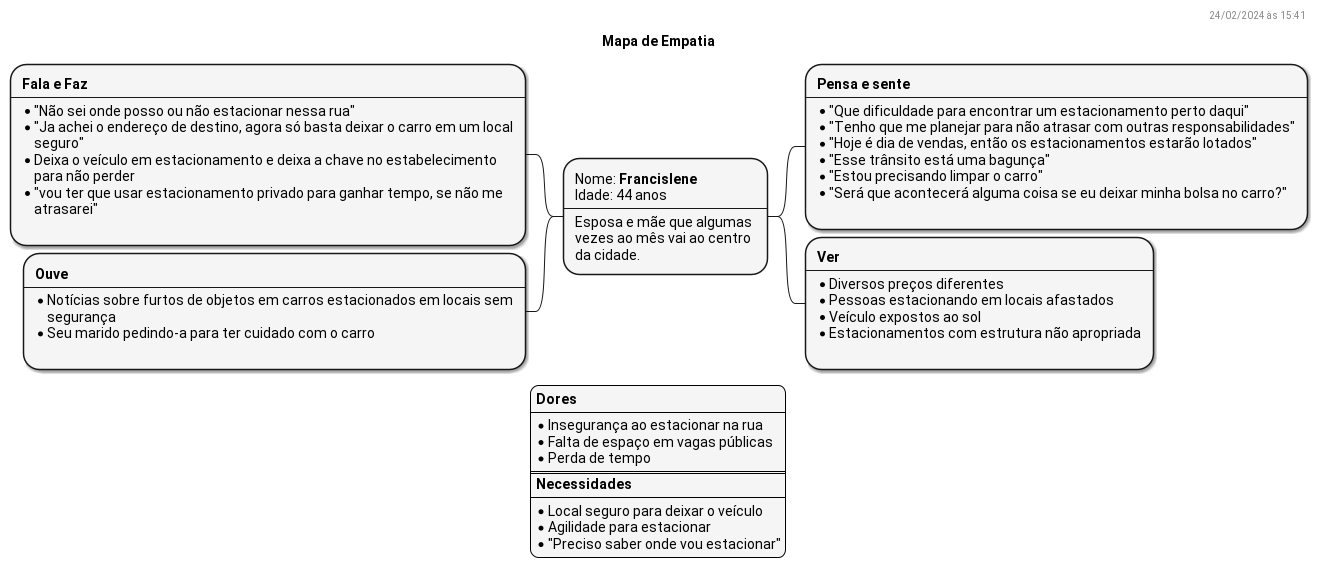
\includegraphics[width=\linewidth]{build/mapa_de_empatia_1_fran.png}}
\end{figure}


% OBSERVAÇÃO: A seção de referências deve ser gerada automaticamente usando os comandos \cite{} do LaTex. Recomenda-se o uso do padrão IEEE para citações, conforme abaixo.
 \newpage
 \bibliographystyle{IEEEtran}
 \bibliography{bibliografia}

\end{document}
